%
% File naacl2019.tex
%
%% Based on the style files for ACL 2018 and NAACL 2018, which were
%% Based on the style files for ACL-2015, with some improvements
%%  taken from the NAACL-2016 style
%% Based on the style files for ACL-2014, which were, in turn,
%% based on ACL-2013, ACL-2012, ACL-2011, ACL-2010, ACL-IJCNLP-2009,
%% EACL-2009, IJCNLP-2008...
%% Based on the style files for EACL 2006 by 
%%e.agirre@ehu.es or Sergi.Balari@uab.es
%% and that of ACL 08 by Joakim Nivre and Noah Smith

\documentclass[11pt,a4paper]{article}
\usepackage[hyperref]{naaclhlt2019}
\usepackage{times}
\usepackage{color}
\usepackage{latexsym}
\usepackage{graphicx}

\usepackage{url}
\usepackage{soul}

%\aclfinalcopy % Uncomment this line for the final submission
%\def\aclpaperid{***} %  Enter the acl Paper ID here

%\setlength\titlebox{5cm}
% You can expand the titlebox if you need extra space
% to show all the authors. Please do not make the titlebox
% smaller than 5cm (the original size); we will check this
% in the camera-ready version and ask you to change it back.

\newcommand{\todo}[1]{{\sethlcolor{green}\hl{#1}}}
\newcommand{\rephrase}[1]{{\sethlcolor{cyan}\hl{#1}}}

\newcommand{\emmatodo}[1]{\textcolor{red}{TODO: #1}}

\newcommand\BibTeX{B{\sc ib}\TeX}

\title{Improved representation learning for semantic role labeling}

\author{First Author \\
  Affiliation / Address line 1 \\
  Affiliation / Address line 2 \\
  Affiliation / Address line 3 \\
  {\tt email@domain} \\\And
  Second Author \\
  Affiliation / Address line 1 \\
  Affiliation / Address line 2 \\
  Affiliation / Address line 3 \\
  {\tt email@domain} \\}

\date{}

\begin{document}
\maketitle
\begin{abstract}
  \emmatodo{write this well} PropBank SRL has a lot of annotation available, and as a result has recently seen a surge in interest and resulting substantial gains in accuracy (over/nearly XX F1) thanks to neural network models. But PropBank core argument labels are designed to generalize across the entire dataset, leading to the same label having different meanings for different predicates: e.g. depending on the predicate, {\sc arg2} may correspond to X different roles such as  \emph{destination} or \emph{extent}. This ambiguity in ProbBank makes learning challenging, and appears to be the cause of much of the remaining mistakes predicted by the best SRL systems: Error analysis of state-of-the-art SRL models has shown that a substantial portion of the errors [give approximate num?] come from otherwise correctly predicted spans that receive incorrect labels. Other frameworks for semantic roles such as VerbNet assign many more fine-grained labels that are consistent across predicates, but this leads to sparsity in the labels, making it difficult to achieve high test-time accuracy. In response we propose a single multi-task model which leverages fine-grained VerbNet annotations to help disambiguate PropBank core argument labels. Our single model is trained to predict both VerbNet and PropBank semantic role labels, and token representations used for PropBank classification are composed from VerbNet label embeddings. We find that incorporating VerbNet into training improves PropBank accuracy [we need to be specific as possible without committing to results we don't have]
\end{abstract}


\section{Introduction}
Semantic role labeling (SRL) is the task of identifying the latent predicate argument structure of a sentence to answer the question 'who' did 'what' to 'whom', 'when', and 'where'. \emmatodo{The semantic formalism with the most annotated data is PropBank \cite{palmer2005proposition}, which...} PropBank defines a verb-specific numbered annotation scheme. For instance, ARG0 for a verb "Accept" corresponds to the proto-typical 'Agent', the "Acceptor" while ARG1 corresponds to the proto-typical 'Patient/Theme', the "Accepted thing". \emmatodo{there has been recent great success in developing SRL models which use the PropBank  semantic representation, leveraging the substantial amount of annotation to train highly accurate deep neural network models [cite: Zhou and Xu 2015, He et al. 2017, Tan et al. 2018, Strubell et al. 2018]. Over the past 5 years, this improved modeling has led to an XX decrease in error, bringing F1 on this task to nearly 90.}

\emmatodo{error analysis has shown that the largest source or errors for state-of-the-art models comes from label confusion on correctly predicted spans. this can be attributed to... } While PropBank is a useful semantic formalism utilized by state-of-the-art SRL systems \cite{strubell2018linguistically}, it defines coarse-grained labels which aren't strictly associated with a role \cite{loper2007combining}.  This is especially evident in arguments from ARG2-ARG5, where the meaning of a role changes across predicates. For example, for the predicate \textit{bring}, the meaning of ARG2 corresponds to \textit{Destination}. However, for the predicate \textit{rise}, ARG2 corresponds to \textit{Extent}. For a supervised model, the distinctions between the core arguments can be difficult to learn because of this phenomenon.

Concretely, on examining the errors made by the model in \cite{strubell2018linguistically}, we find that labeling errors overall contribute to a drop of about 5.8 F1 absolute on the \rephrase{CoNLL-2012 shared task}. Of these, confusion among the core arguments from ARG0-ARG5 in PropBank constitute around 31\% of the labeling errors. In order to reduce these errors, we need labels that are consistent across predicates. VerbNet \cite{schuler2005verbnet} satisfies these constraints, providing consistent, finer-grained labels such as Agent, Theme, Instrument, etc. \todo{However, since VerbNet doesn't generalize well to unseen predicates, and since it is much sparser than PropBank annotations, we still want to learn and predict PropBank labels.}

In repsonse, we propose a multi-task neural network architecture which leverages fine-grained VerbNet role labels to compose a better representation for PropBank roles, and consequently, learn to make better predictions on the PropBank labels.
%method to integrate the information from the VerbNet labels into the multi-tasking model for SRL described in \cite{strubell2018linguistically} (LISA). 
We do this by \emmatodo{describe in more detail how we do it.}

In experiments on the CoNLL-2012 SRL benchmark, we show \emmatodo{summary of results go here}

\section{Model}
\emmatodo{don't start this by talking about the LISA model, talk about OUR model (which is based on SA from LISA paper)}
The LISA model \cite{strubell2018linguistically} combines multi-head self-attention with multi-task learning across dependency parsing, part-of-speech tagging, predicate detection and SRL. We add the task of predicting VerbNet labels for semantic roles as an additional task into this model.

To explicitly incorporate the new labels, we use the predictions on the VerbNet task to form a role representation for each VerbNet role. We then add the VerbNet representation to the PropBank role representation to get an auxiliary role representation that is then scored against each predicate. The details of each component are described below.

\subsection{Self-attention for semantic role labeling \label{sec:self-attn}}

\emmatodo{describe our basic model here (which is really the SA model from \citep{strubell2018linguistically}). Basically you want to say that it takes pre-trained word embeddings as input, concatenated with predicate indicator embedding. These representations are passed through $L$ (or whatever variable name) layers of self-attention in the style of the encoder of Vaswani et al. (2017)). These are passed to a bilinear scoring function... [an earlier layer is trained to predict parts-of-speech?] The variables to be defined are the ones that we need in order to explain the changes that we made (next two sections), so I think that'll just mean the final encoded token representations (output of transformer), and the bilinear stuff (again, just what you need to explain the next two sections -- writing those first should inform how much detail (math specifically) you need here. }

\subsection{Predicting VerbNet roles}
\emmatodo{in this section just talk about how we add verbnet role prediction as another task, and we do it in the same way as propbank roles are predicted in baseline model described in \S\ref{sec:self-attn}}
For each VerbNet class, we learn an embedding of dimension $d$, which yields a label embedding matrix of size $c_{vn} * d$ where $c_{vn}$ is the number of VerbNet classes. 

Similar to the LISA model, each token representation $s_t$ is projected to a predicate representation $s_t^{pred}$ and a role representation $s_t^{role}$. Then, for each VerbNet class, a score is produced by the model for every token. Using the per-class scores for each token as attention weights, we form an attended representation $v_t^{role}$ of size $d$ from the label embedding matrix.

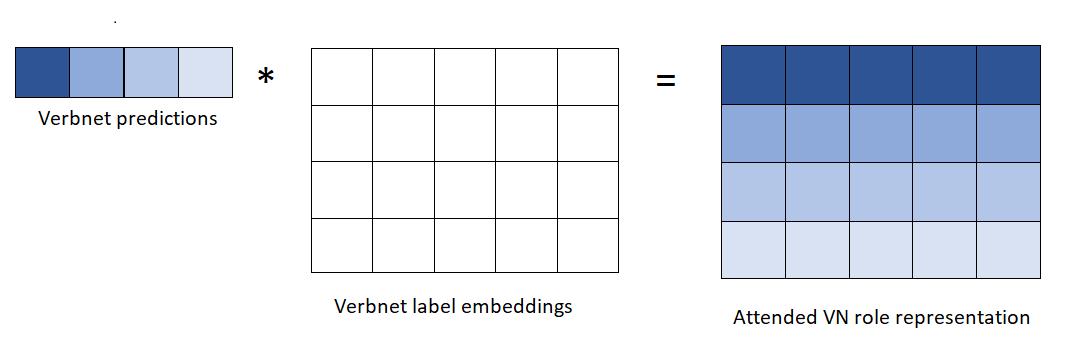
\includegraphics[scale=0.4]{model.PNG}

\subsection{Composed representation}
\emmatodo{better title for this important/central section}
For the task of predicting PropBank roles, we have another copy of the predicate representation $s_t^{pred}$ and role representation $s_t^{role}$ where the latter is of size $d$. We add $v_t^{role}$ to $s_t^{role}$ to get a single representation, $w_t^{role}$ that encapsulates information from PropBank and VerbNet. \emmatodo{HERE is where you def need to have the equations}

This composed representation is then used for making predictions for the PropBank SRL prediction task as described in \S\ref{sec:self-attn}.

\subsection{Training}
\emmatodo{describe how we do training here: where we use gold vs. predicted representations, which things are masked, perhaps (i.e. for verbnet we only train and say that the loss is just the sum of the separate losses, maybe with a penalty.}

\section{Related Work}

\section{Experimental results}

\emmatodo{summarize experimental results here, describe the baselines/experiments in brief}

\subsection{Data and preprocessing}
The SemLink dataset \cite{palmer2009semlink} \emmatodo{describe the dataset more precisely}. We map the annotations in SemLink to the corresponding sentences in the newswire (nw) portion of the CoNLL-2012 shared task [cite], filtered for sentences which contain predicates following [cite he et al. 2018]. \emmatodo{add more detail here regarding how we handled all the edge case stuff -- e.g. labeled in semlink but with no verbnet}
%to obtain  to get mappings between PropBank and VerbNet for the \rephrase{Wall Street Journal portion of OntoNotes.} 
This gives us 9149 sentences, containing a total of 238054 tokens, and 55419 predicates, that have both PropBank and VerbNet annotations for semantic roles. \emmatodo{break down by train/dev/test, or at least, most importantly, specify train numbers, or that these are overall... i would maybe say overall and train numbers.}

\subsection{CoNLL-2012}

\emmatodo{put main results here: ideally, want baseline (no verbnet), multitask w/ verbnet, and our shared representation thing. All using gold predicates, ideally re-encoding sequence WRT each predicate. And, with glove and ELMo embeddings.}

\subsection{Error analysis}

\emmatodo{here is where we include confusion matrix and other analysis (can use luheng's amazing scripts), and hopefully show that we reduced the errors we were trying to reduce.}

\section{Conclusion}

%\section*{Acknowledgments}

%The acknowledgments should go immediately before the references.  Do
%not number the acknowledgments section. Do not include this section
%when submitting your paper for review. \\

\bibliography{naaclhlt2019}
\bibliographystyle{acl_natbib}

\appendix

\section{Supplemental Material}
\label{sec:supplemental}

\end{document}
